%%%%%%%%%%%%%%%%%%%%%%%%%%%%%%%%%%%%%%%%%%%%%%%%%%%%%%%%%%%%%%%%%%%%%%%%%%%%%%%%%%%%%%%%
\section{Neural Network Diagrammatics}
\label{section:neural-network-diagrammatics}
%%%%%%%%%%%%%%%%%%%%%%%%%%%%%%%%%%%%%%%%%%%%%%%%%%%%%%%%%%%%%%%%%%%%%%%%%%%%%%%%%%%%%%%%
%
%
\subsection{Linear Regression}
%
%
We start by reframing our linear regression model as a very simple neural network.
In doing so, we can start to introduce some new terminology and elements of the diagrammatic language used to describe neural network architectures.
%
\begin{figure}[H]
    \centering
    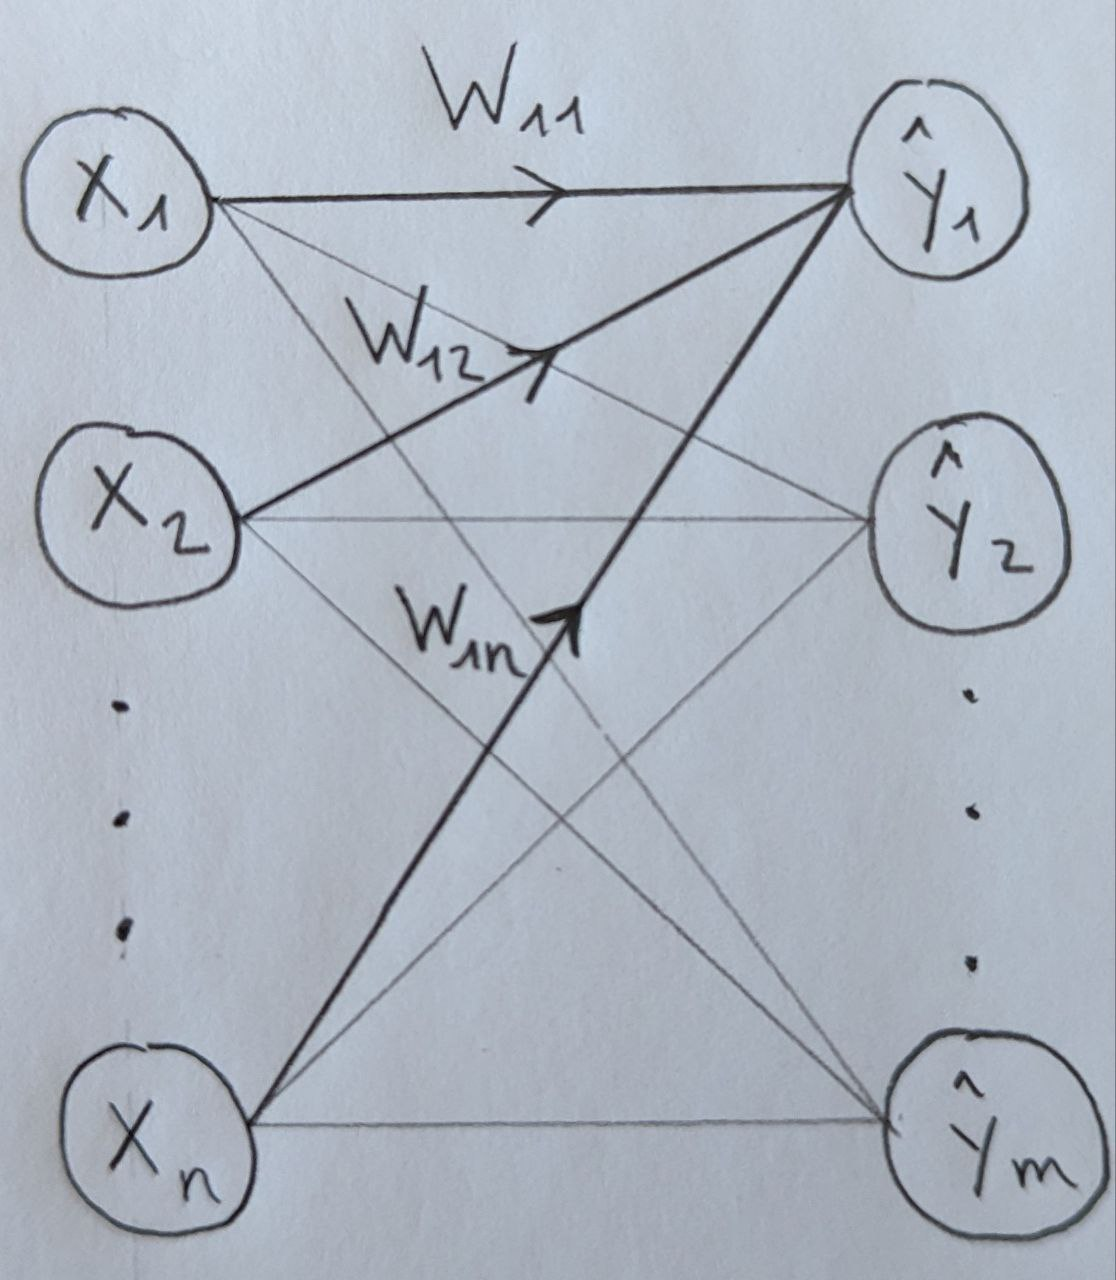
\includegraphics[width=0.5\textwidth]{../figures/chapter_01/nn_diagram_linear_regression.png}
\end{figure}
%

The arrows connecting the input, $\bx$, to the output, $\hat{\by}$, represent matrix multiplication by the weights matrix, $W$.
A summation over all arrows flowing into a node is implied.
With this in mind, the figure can be seen as a diagrammatic representation of the model, $f(\bx ~|~ W) = W \bx$.
Unless stated otherwise, we will use the convention that we read such diagrams from left to right.

%
%
\subsection{Binary Classification and Logistic Regression}
%
%
Let's now draw a slightly more interesting neural network diagram suited to solving a different type of problem.
Once again, we have a set of measurements $\{(\bx^{(k)}, y^{(k)})\}_{k=1}^K$, but now $y^{(k)} \in \{0, 1\}$, \ie, we are dealing with two classes labeled by the integers $0$ and $1$.

If we were to apply a linear model, our output would fall anywhere on the real line, which is clearly not what we want.
In principle, we could come up with a rule $h: \RR \rightarrow \{0, 1\}$ which maps from the output of our linear model to the target space.
This idea of adding non-linearity to our model is a good one, but there is a method better suited to this type of problem, namely, \textit{logistic regression}.
We will still need some rule to map exactly to our target space, but rather than mapping from the real line, we could have a model which produces an output in the interval $(0, 1)$, which we can interpret as the probability of belonging to one of our classes.
The function we choose to do this with is called the \textit{logistic function}\footnote{Actually, this is the \textit{standard} logistic function, which has a few constants fixed to special values. Though the standard logistic function is a specific example of a \textit{sigmoid function}, it is sometimes referred to simply as \textit{the} sigmoid function.}, and it is defined as
%
\begin{equation}
    \sigma(z) = \frac{1}{1 + e^{-z}}.
\end{equation}
%

With this function in hand, we are now prepared to diagram our model:
%
\begin{figure}[H]
    \centering
    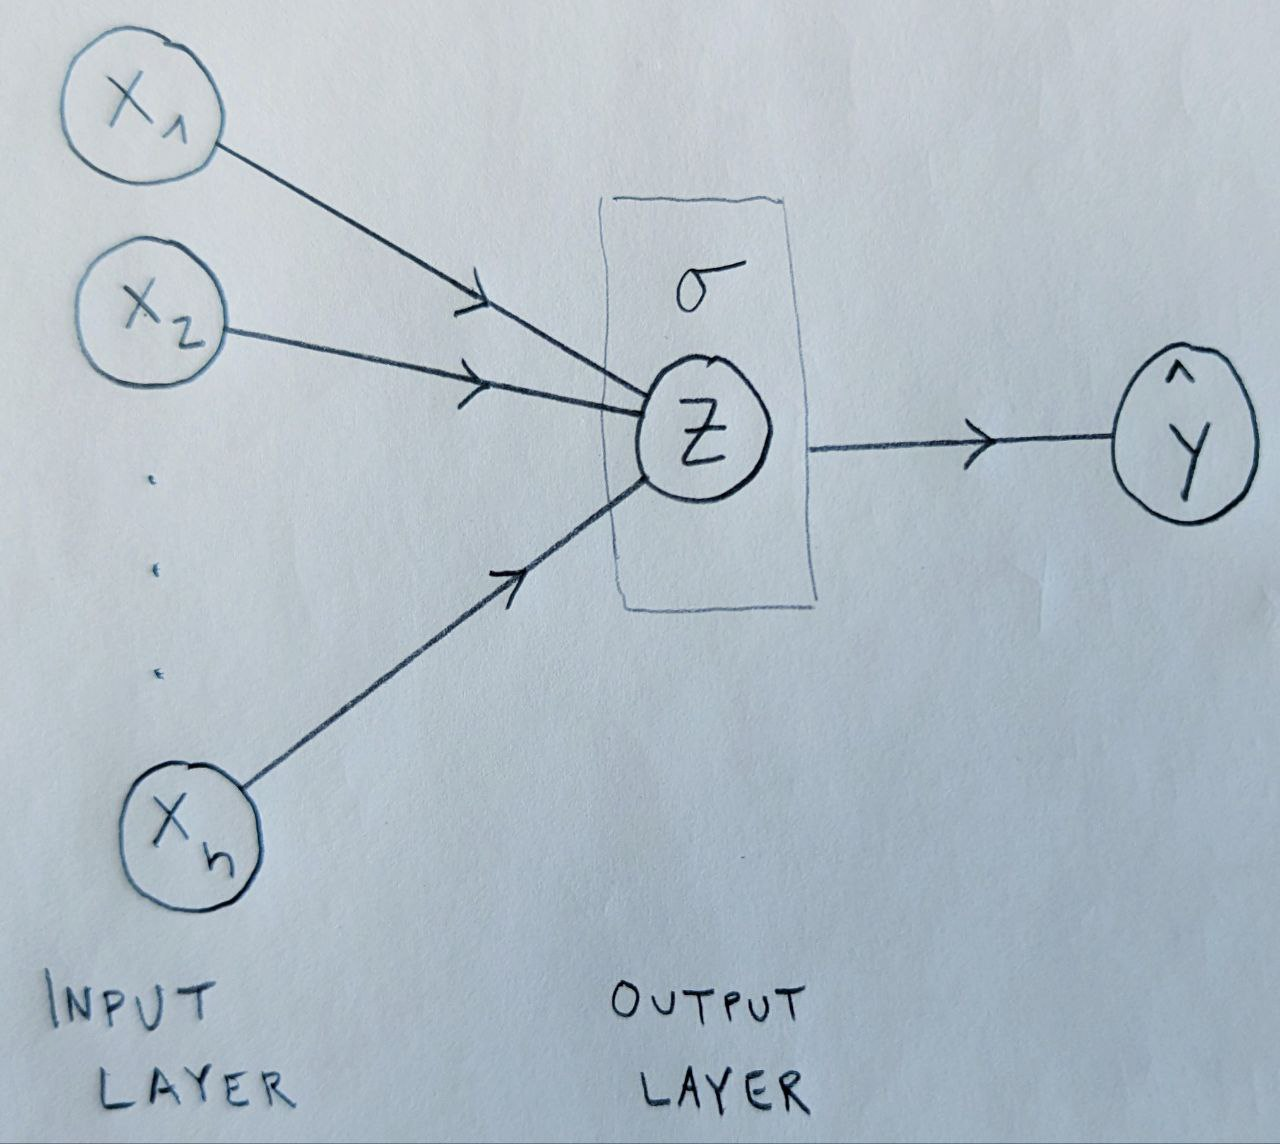
\includegraphics[width=0.5\textwidth]{../figures/chapter_01/nn_diagram_logistic_regression.png}
\end{figure}
%
\noindent Translating this to an equation, the model reads $f(\bx ~|~ W) = \sigma(W \bx)$.
We have also introduced some nomenclature here, namely, the idea of an input layer and an output layer.
The input layer is merely the first layer, which takes the independent variable and feeds it into the model.
The output layer is then the final layer, which produces the final model output.

The final missing piece of the puzzle is an appropriate loss function.
Mean squared error is not really appropriate for this application, rather, we need a loss function which, when minimized, will produce a model which can be interpreted as the probability that our measurement belongs to a certain class.
Glossing over the details of the maximum likelihood method and Bernoulli distributions, we take the so-called \textit{log-loss} to be our loss function,
%
\begin{equation}
    \mathcal{L}\left(\{(\bx^{(k)}, y^{(k)})\}_k ~\big|~ f\right) =
    -\sum_{k=1}^K \left[y^{(k)} \ln{f(\bx^{(k)}) + (1 - y^{(k)}) \ln{(1 - f(\bx^{(k)}))}}\right].
\end{equation}
%

Written in this way, our model $f(\bx)$ represents the predicted probability that a given measurement belongs to the class labeled $1$.
We are now free to choose a rule to map this probability to our discrete target space, \eg, by introducing a cutoff probability. 

%
%
\subsection{Multi-Label Classification and the \textit{softmax} Function}
%
%
Suppose we wish to allow our measurements to belong to an arbitrary number of classes, $m \in \NN$, \ie, our dependent variable $\by$ is an $m$ dimensional vector, where the $i^{\rm th}$ component $y_i = \delta_{ij}$ denotes the measurement belonging to class $j$.
We wish to construct a model which produces a probability distribution over our $m$ classes,
%
\begin{equation}
    f(\bx) = \hat{\by}, \quad \text{where}\quad \hat{y}_i \in (0, 1)\quad \text{and}\quad \sum_{i=1}^m \hat{y}_i = 1.
\end{equation}
%
To do this, we will need an appropriate non-linear function to properly constrain our output \textit{and} an appropriate loss function.

A basic model which achieves this could look as follows:
%
\begin{figure}[H]
    \centering
    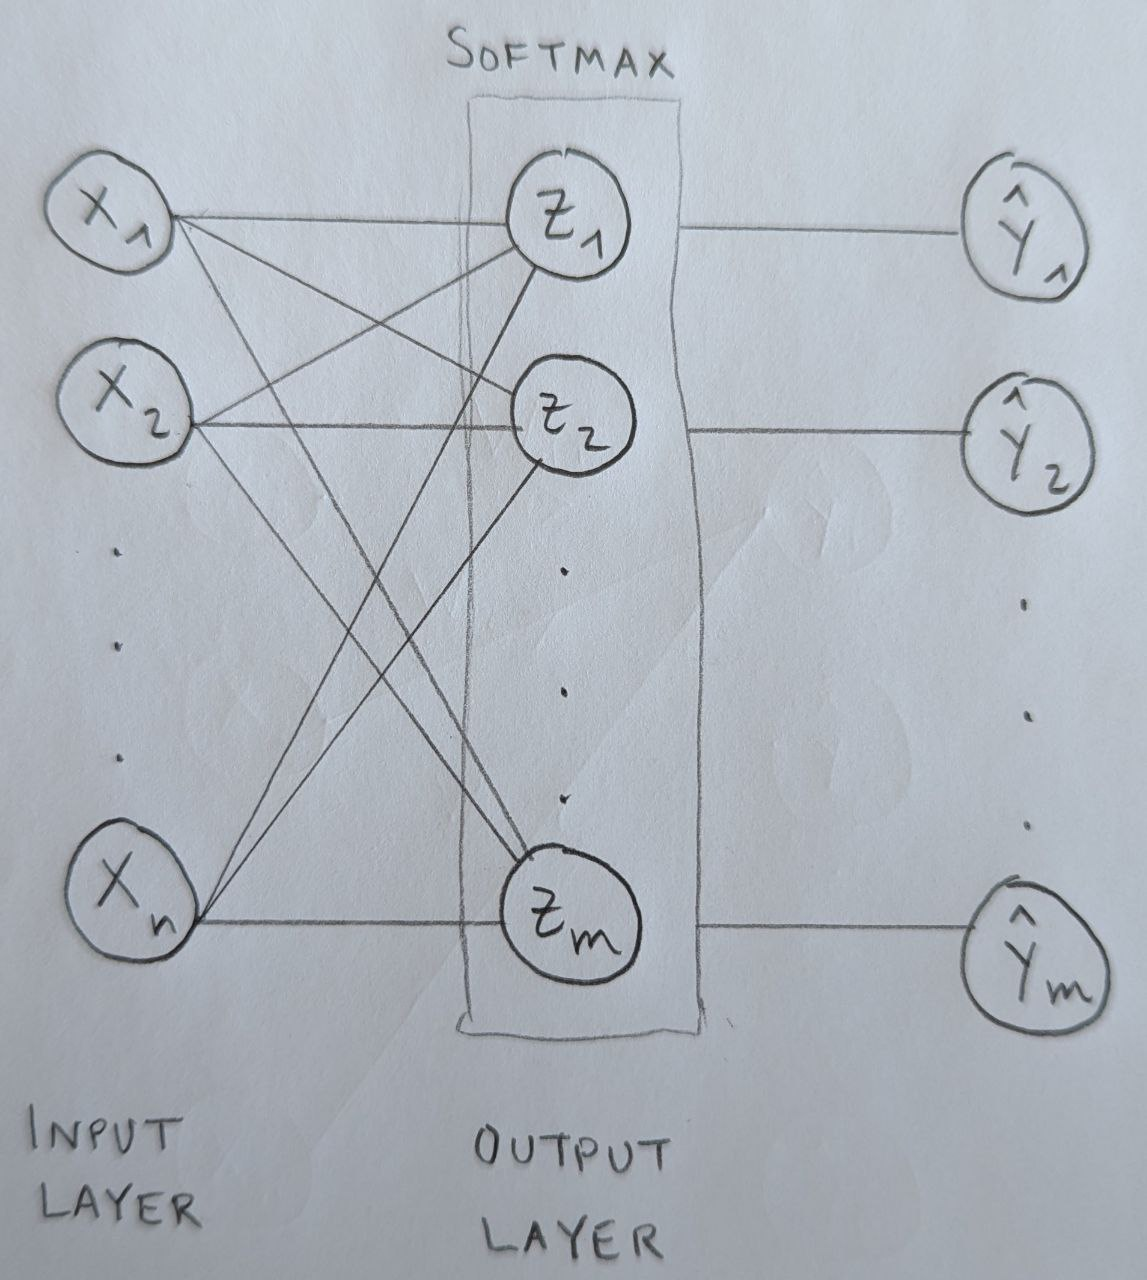
\includegraphics[width=0.5\textwidth]{../figures/chapter_01/nn_diagram_multilabel_classifier.png}
\end{figure}
%
The transformation in the output layer is called $\softmax$ and it is defined as
%
\begin{align}
    \softmax: ~\RR^m &\rightarrow (0, 1)^m \nonumber\\
              ~\bz   &\mapsto \sum_i \frac{e^{z_i}}{\sum_j e^{z_j}} \hat{\be}_i
\end{align}
%
and can easily be seen to satisfy the necessary normalization conditions.
The model may then be written down as
%
\begin{equation}
    f(\bx ~|~ W) = \softmax(W \bx).
\end{equation}
%

The appropriate loss function which allows for the interpretation of our model as a probability distribution over the $m$ classes is a generalization of the log-loss used above called the \textit{cross entropy},
%
\begin{equation}
    \mathcal{L}\left(\{(\bx^{(k)}, \by^{(k)})\}_k ~\big|~ f\right) = -\sum_{k=1}^K \sum_{i=1}^m y^{(k)}_i \ln \left[f(\bx^{(k)})\right]_i.
\end{equation}
%

%
%
\subsection{Hidden Layers, Non-Linearity and Model Complexity}
%
%
Now that we have these diagrammatics, it seems rather trivial to add additional layers between the input and output layers to make a more complex model.
Is this really the case?

Yes, but with a caveat. Consider the model in the following diagram:
%
\begin{figure}[H]
    \centering
    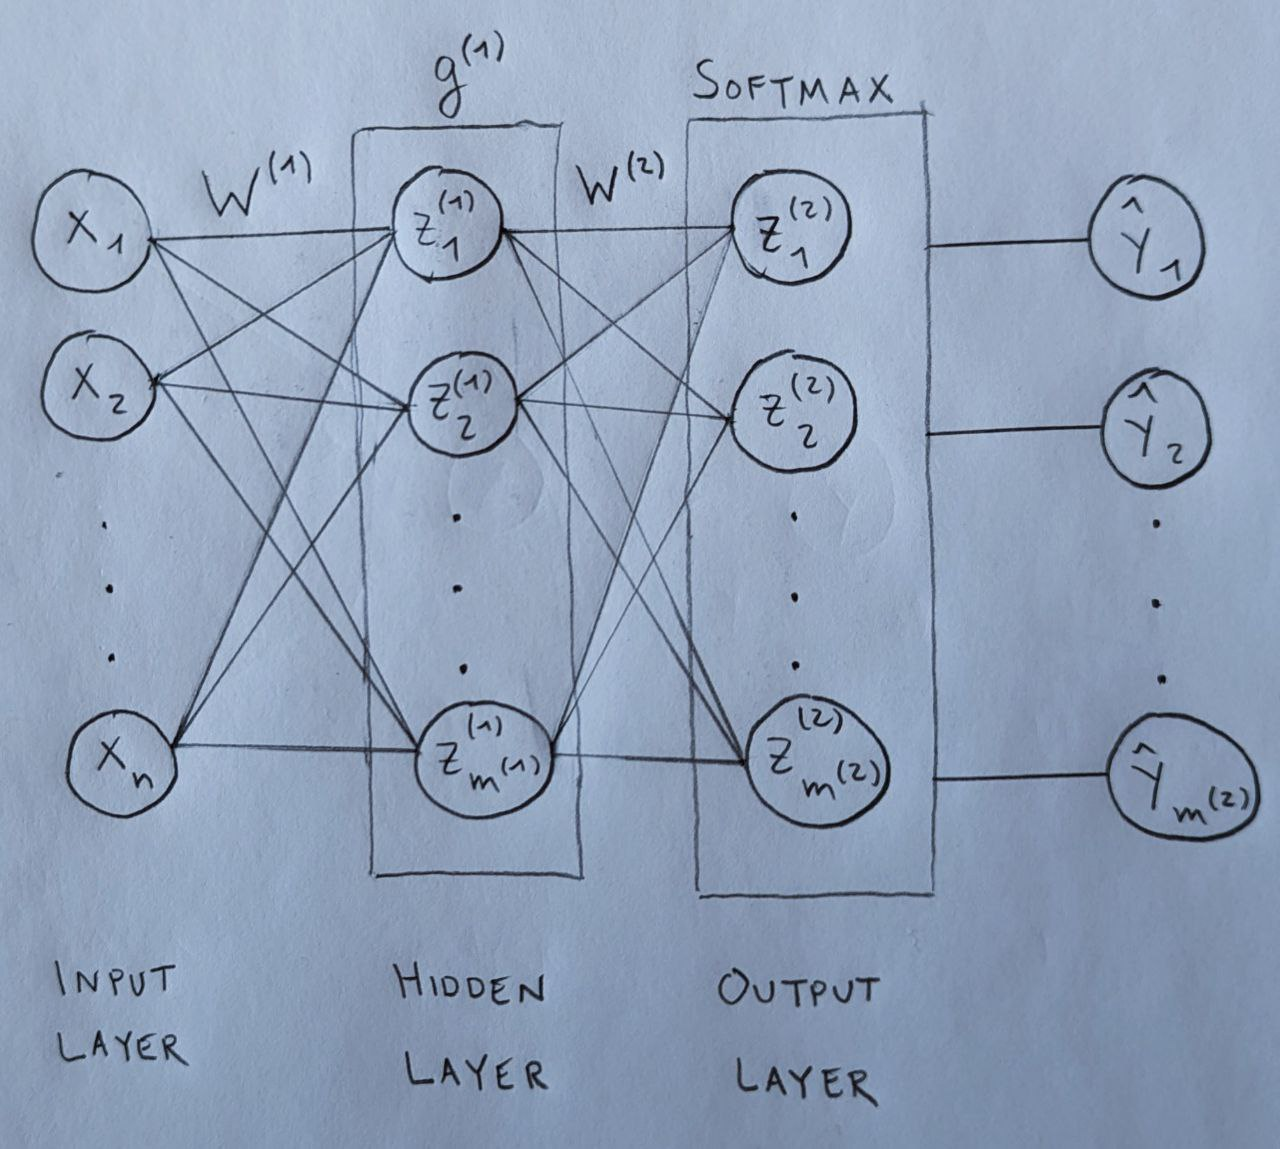
\includegraphics[width=0.5\textwidth]{../figures/chapter_01/nn_diagram_hidden_layers.png}
\end{figure}
%
\noindent Here, we have added a so-called \textit{hidden layer} between the input and output layers.
Ignoring for a moment the $g^{(1)}$ above the hidden layer, this diagram would translate to a model
%
\begin{equation}
    f(\bx ~|~ W^{(1)}, W^{(2)}) = \softmax(W^{(2)} W^{(1)} \bx),
\end{equation}
%
In defining this model, we have added a second matrix multiplication step compared to the model in the last section.

Have we gained anything by doing so?
Sadly, no.
To see this, define a matrix $W = W^{(2)} W^{(1)}$ and note that the model above may be written simply as
%
\begin{equation}
    f(\bx ~|~ W) = \softmax(W \bx),
\end{equation}
%
\ie, we may collapse the input layer and the hidden layer into a single input layer with weights matrix $W$, and we have the exact same model as in the last section.
All we have done by introducing this hidden layer is to store (and eventually optimize) some addition parameters and to perform some unnecessary matrix multiplication.
Our problem is that the composition of multiple linear (affine) transformations is, itself, just a linear (affine) transformation.
Nothing can be gained by adding additional hidden layers that only perform linear transformations.

We \textit{can}, however, add model complexity if we include a non-linearity to these layers by introducing a so-called \textit{activation function}.
For the $i^{\rm th}$ hidden layer, we compose the corresponding linear transformation, $W^{(i)}$, with a non-linear activation function, $g^{(i)}$, before sending it off to the next layer.
If we now stop ignoring the activation function in the last diagram, we see that the model really reads
%
\begin{equation}
    f(\bx ~|~ W^{(1)}, W^{(2)}) = \softmax(W^{(2)} g^{(1)}(W^{(1)} \bx)).
\end{equation}
%
In general, the activation functions are understood to operate on each component of their input individually, \ie,
%
\begin{align}
    g^{(i)}: ~\RR^{m^{(i)}}   &\rightarrow \RR^{m^{(i)}} \nonumber\\
                   ~\bz^{(i)} &\mapsto \sum_{\mu = 1}^{m^{(i)}} g^{(i)}(z^{(i)}_\mu) \hat{\be}_\mu.
\end{align}
%
